\documentclass{article}

\usepackage{geometry}
\usepackage{gbt7714}
\usepackage{xeCJK}
\usepackage{booktabs}       % professional-quality tables
\usepackage{amsfonts}       % blackboard math symbols
\usepackage{subfig}
\usepackage{amsmath}
\usepackage{graphicx}
\usepackage{float}
\usepackage{svg}

\graphicspath{{assets/}}


\linespread{1.5}
\geometry{a4paper, left=2.5cm, right=2.5cm, top=2.5cm, bottom=2.5cm}
\bibliographystyle{gbt7714-numerical}   
\title{基于软约束潜在正则化对抗的高压并联电抗器异常声音检测}

\begin{document}
\maketitle

\begin{abstract}
  本文提出了一种软约束潜在正则化对抗异常检测方法(Soft-LRAAD),旨在解决LRAAD方法中超参数M对生成器生成频谱图的KL散度上限的硬约束带来的问题。LRAAD方法使用硬约束来控制KL散度上限,这样不仅使模型难以将正常数据和异常数据在潜在空间中进行有效分离,而且会导致模型训练不稳定,进而影响模型性能。
  为了解决这一问题,Soft-LRAAD方法引入了软约束损失替代硬约束损失,即使用一个平滑的函数来逼近KL散度的上限约束损失。通过这种方式,Soft-LRAAD方法提高了模型在潜在空间中区分正常数据和异常数据的能力,同时增强了模型训练的稳定性,从而提升了整体性能。
本文在变电站实测声音数据集上进行了实验验证,结果显示Soft-LRAAD方法在异常检测任务上的AUC指标明显优于其他基线模型,验证了该方法的有效性和实用性,为异常声音检测在高压电抗器态监测领域提供了新的解决方案。
\end{abstract}


关键字:声学异常检测, 半监督学习, 对抗学习, 潜在变量正则化对抗

\section{引言}

高压并联电抗器在特高压变电站中起着至关重要的作用,其主要功能是补偿无功功率,稳定电网电压,防止电力系统中过电压的发生\cite{das2017novel,magdaleno2014temperature,tumay2017review}。由于特高压变电站运行环境复杂,高压并联电抗器在长期运行过程中可能会出现各种故障,例如电弧放电、绕组松动、机械振动等\cite{yao2015noninvasive,velasquez2019root}。这些故障往往伴随着异常的声音信号,因此对高压并联电抗器进行异常声音检测,对于保障电力系统的安全和可靠性具有重要意义。

目前,针对高压并联电抗器的异常检测方法主要包括油色谱检测、超声局放检测和高频局放检测。这些方法虽然在一定程度上能够帮助识别设备内部的潜在故障,但也存在着一些局限性:

\begin{enumerate}

  \item{\textbf{油色谱检测:}油色谱检测是一种成熟的故障诊断方法,主要通过分析油中的气体组分来判断设备内部是否存在放电或过热问题\cite{ali2023conventional}。尽管油色谱分析能够提供关于放电或过热故障的早期预警信息,但其检测周期较长,实时性差,且难以反映电抗器的瞬时状态变化。此外,油色谱检测对早期和微小故障的敏感度较低,可能导致故障在发展到较严重阶段时才被检测到。}

  \item{\textbf{超声和高频局放检测:}超声检测通过捕捉电抗器内部局部放电产生的超声波信号来检测异常\cite{wang2018partial},高频检测利用高频电磁波信号检测电抗器内部的局部放电现象\cite{zheng2020feasibility}。这些方法在检测高压设备中的局部放电方面具有较高的灵敏度,尤其是在设备内部绝缘材料老化或发生局部放电时可以提供较为准确的诊断结果。然而,这些方法的检测精度和灵敏度容易受到环境噪声和外部干扰的影响,尤其是在复杂的电磁环境中,检测结果可能存在不稳定性。此外,超声和高频局放检测在检测机械故障和设备的振动问题时,效果较为有限,难以全面反映高压并联电抗器的运行状态。}

\end{enumerate}

相比之下,基于声学信号的检测方法能够同时监测设备运行中的机械和电气故障,且不受油质变化和局放信号的限制,具有更强的实时性和鲁棒性\cite{ilkhechi2021applications,gao2022early}。本文提出的Soft-LRAAD方法通过软约束潜在正则化对抗异常检测技术,结合深度学习模型在声学信号分析中的优势,能够有效提高高压并联电抗器故障检测的精度和可靠性。

随着人工智能技术的快速发展,基于数据驱动的异常检测方法逐渐成为研究热点。近年来,深度学习技术在图像识别、语音处理等领域取得了显著成果,这为高压并联电抗器的异常检测提供了新的思路。特别是对抗学习(Adversarial Learning)和潜在变量模型(Latent Variable Models)的结合,能够有效地提取数据的深层次特征,实现对异常模式的高精度识别。然而,现有的对抗学习方法,如潜在正则化对抗异常检测(LRAAD),在应用于高压并联电抗器的异常检测时,仍存在一些问题。LRAAD方法通过硬约束来控制潜在空间的KL散度上限,这种硬约束虽然可以帮助模型在潜在空间中区分正常数据和异常数据,但也容易导致模型在训练过程中出现不稳定性,影响最终的检测效果。此外,硬约束的引入还可能使得生成的潜在空间不够灵活,难以捕捉异常数据的多样性和复杂性。

为了解决这些问题,本文提出了一种基于软约束潜在正则化对抗学习的高压并联电抗器异常检测方法(Soft-LRAAD)。该方法通过引入软约束损失函数,替代LRAAD方法中的硬约束损失,从而在潜在空间中更为灵活地处理正常数据和异常数据的分布问题。这种改进不仅提高了模型的训练稳定性,也增强了模型在不同工况下的异常检测性能。此外,本文在特高压变电站的实测声音数据集上,对所提出的方法进行了实验验证,结果表明,Soft-LRAAD方法在异常检测任务中表现出优异的性能,显著优于传统方法。


本文的主要贡献包括以下几点:

\begin{enumerate}

  \item 提出了异常检测方法Soft-LRAAD,通过软边界的方式来控制生成器生成频谱图的KL散度上界,极大程度提高来正常数据和异常数据的在潜在空间的分离效果,从而提高了异常检测的准确性和鲁棒性。

  \item 设计了基于KL散度损失和重构损失的异常分数,相比与仅使用重构损失作为异常分数的方法,基于KL散度和重构损失的异常分数能够更好地区分正常数据和异常数据,提高了异常检测的性能。

  \item 使用特高压变电站的实测声音数据对模型进行了验证,实验结果表明,Soft-LRAAD方法在不同负载条件下均表现出较高的异常检测准确率和鲁棒性。

\end{enumerate}

本文的结构安排如下:第二章介绍了相关研究工作和背景知识;第三章介绍了LRAAD模型的背景知识,第四章详细描述了Soft-LRAAD模型的设计和实现,包括编码器和生成器的架构及其训练方法;第五章介绍了实验设置和数据集划分,并对实验结果进行分析和讨论;第六章总结了本文的研究工作,并提出了未来的研究方向。

\section{相关工作}

过去的研究已经涵盖了多种声学异常检测方法和相关技术。其中,一些方法依赖于传统的信号处理技术,而另一些方法则利用了深度学习和人工智能等新兴技术\cite{mnasri2022anomalous, jombo2023acoustic}。基于传统信号处理的方法通常包括特征提取、模式识别和分类等步骤。这些方法通常包括使用滤波器、时频分析、频谱分析等技术来提取声音信号的特征,并使用分类器(如支持向量机、k最近邻等)来识别异常。尽管传统方法在某些情况下取得了一定的成果,但其局限性在于依赖于人工特征设计和手动调整参数,且难以处理复杂的非线性关系和大规模数据\cite{pang2021deep, chalapathy2019deep, shi2021equipment}。

近年来,随着深度学习技术的发展,基于潜在变量模型的方法在电力设备声学异常检测领域取得了显著的进展\cite{AE-AD,AE-AD-2,CAE-AD,VAE-AD,VAE-AD-2,SAE-AD}。Duman等人\cite{CAE-AD}提出了一种基于卷积自编码器(CAE)的工业过程声学异常检测方法。该方法使用对数刻度的Mel频谱特征作为模型的输入特征。与传统的异常检测方法One-Class Support Vector Machine(OCSVM)\cite{ocsvm}相比,CAE方法在工业过程中表现出更好的异常检测效果。基于变分自编码器(VAE)的异常检测方法\cite{VAE-AD,VAE-AD-2}通过引入潜在变量和KL散度来学习数据的潜在表示,从而提高模型的泛化能力。例如,An等人\cite{VAE-AD}提出了一种基于变分自编码器的异常检测方法,该方法通过训练一个VAE模型来学习正常数据的潜在表示,然后使用KL散度来衡量正常数据和异常数据之间的差异。
%近年来,学生-教师方法在异常检测领域的应用也得到了广泛的关注。Zhang等人\cite{destseg}提出了DeSTSeg模型,包括一个预训练的教师网络、一个去噪学生网络和一个分割网络。模型的训练分为两个步骤,首先使用合成的异常图像作为学生网络的输入,使用原始的干净图像作为教师网络的输入,通过优化分割网络的参数来定位异常区域。然后,在推理阶段,通过后处理生成像素级别的异常图,并计算相应的图像级别的异常分数。Batzner等人\cite{efficientad}提出了EfficientAD方法,该方法使用预训练神经网络从图像中提取特征,并使用轻量级的学生-教师模型在测试时检测异常特征。此外,论文还介绍了一种用于训练学生-教师模型的新型损失函数。


基于生成对抗网络的异常检测方法在图像异常检测领域取得了显著的进展。文献\cite{anogan}提出了一种基于生成对抗网络(GANs)的异常检测方法,通过对正常样本进行建模来识别异常。f-AnoGAN\cite{f-anogan}在AnoGAN\cite{anogan}方法的改进,AnoGAN使用迭代方法寻找图像在潜在空间的表示,f-AnoGAN通过学习从图像到潜在空间的映射,显著提高了速度。文献\cite{ganomaly}提出了一种名为GANomaly的新型编码器-解码器-编码器架构模型,其同时使用重构损失、潜在表示损失和对抗损失来训练模型和进行异常分数计算,实验表明,其性能优于当代最先进的基于GAN和传统自编码器的异常检测方法,具有泛化到任何异常检测任务的能力。Jiang等人\cite{AEGAN-AD}提出了一种利用生成对抗网络(GAN)进行机器音频异常检测的无监督模型AEGAN-AD。研究表明,通过引入鉴别器来提供特征级别的指导,AEGAN-AD模型可以更深入地理解表示,而不仅仅关注表面噪音,解决了CAE可能会重构出异常信号的问题和WaveNet训练和预测时间长的问题。实验结果显示,该AEGAN-AD模型在DCASE 2022挑战中取得了优异的表现,达到了最先进的性能水平。

LRAAD模型结合了对抗学习和潜在变量模型的优势,能够有效地提取数据的深层次特征,实现对异常模式的高精度识别。然而,LRAAD方法中硬约束的引入容易导致模型训练不稳定,影响最终的检测效果。为了解决这一问题,本文提出了一种基于软约束潜在正则化对抗学习的高压并联电抗器异常检测方法(Soft-LRAAD)。Soft-LRAAD方法通过软约束损失替代硬约束损失,提高了模型在潜在空间中区分正常数据和异常数据的能力,增强了模型训练的稳定性,从而提升了整体性能。

\section{背景}

\textbf{证据下界}:证据下界(Evidence Lower Bound,ELBO)是变分自编码器(Variational Autoencoder,VAE)中的一个重要概念,用于衡量潜在变量的分布与真实分布之间的差异。ELBO由两部分组成,一部分是重构误差,用于衡量生成器生成的数据与原始数据之间的差异;另一部分是KL散度,用于衡量潜在变量的分布与先验分布之间的差异。通过最大化ELBO,可以使得生成器生成的数据更加接近真实数据,同时潜在变量的分布更加接近先验分布。证据下界的公式如下:

\begin{equation}
  ELBO(x)=\mathbb{E}_{q_{\phi}(z \mid x)}[\log p_{\theta}(x \mid z)]-D_{\mathrm{KL}}\left(q_{\phi}(z \mid x) \| p(z)\right) 
\end{equation}

\textbf{LRAAD}:潜在正则化对抗异常检测(Latent Regularized Adversarial Anomaly Detection,LRAAD)是一种基于对抗学习的异常检测方法,通过编码器和生成器来学习正常数据的潜在表示,并通过对抗学习的方式来区分正常数据和异常数据。LRAAD模型的核心思想是通过最小化正常数据的潜在表示与标准正态分布之间的KL散度,来学习将正常数据映射到潜在空间中的正态分布,同时将异常数据映射到潜在空间中的非正态分布。通过这种方式,LRAAD模型可以更好地区分正常数据和异常数据,从而实现异常检测的目的。


\begin{figure}[H]
    \centering
    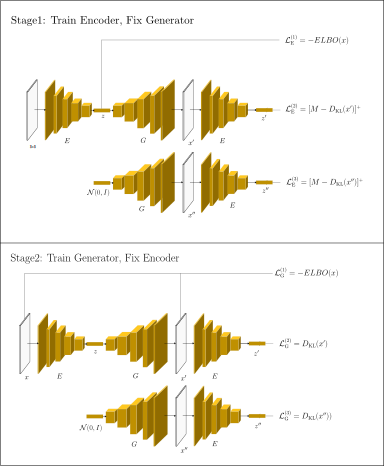
\includegraphics[width=\textwidth]{./assets/lraad.pdf}
    \caption{The Training Pipeline of LRAAD}
    \label{fig:lraad}
\end{figure}

\begin{figure}[H]
    \centering
    \includegraphics[width=\textwidth]{./assets/soft_lraad_model.pdf}
    \caption{The Training Pipeline of Soft-LRAAD}
    \label{fig:soft_lraad}
\end{figure}

记$D_{\mathrm{KL}}(x) = D_{\mathrm{KL}}(q(\cdot \mid x) \| p(\cdot))$。其中,$q(\cdot \mid x)$表示编码器编码频谱图$x$的潜在表示的分布,$p(\cdot)$表示标准正态分布,记为$\mathcal{N}(0, I)$,$D_{\mathrm{KL}}$表示KL散度。


\begin{equation}
  \mathcal{L}_{\mathrm{E}}=\left\|x-x^{\prime}\right\|^2 + D_{\mathrm{KL}}(x) + [M - D_{\mathrm{KL}}(x^\prime)]^{+} + [M - D_{\mathrm{KL}}(x^{\prime\prime})]^{+}
\end{equation}

\begin{equation}
  \mathcal{L}_{\text {G}}= \left\|x-x^{\prime}\right\|^2 + D_\mathrm{KL}(x^\prime) + D_\mathrm{KL}(x^{\prime\prime}))
\end{equation}

等价地,

\begin{equation}
  \mathcal{L}_{\mathrm{E}}=-ELBO(x) + [M - D_{\mathrm{KL}}(x^\prime)]^{+} + [M - D_{\mathrm{KL}}(x^{\prime\prime})]^{+}
\end{equation}

\begin{equation}
  \mathcal{L}_{\text {G}}=-ELBO(x) + D_\mathrm{KL}(x^\prime) + D_\mathrm{KL}(x^{\prime\prime}))
\end{equation}

其中,$[M - D_{\mathrm{KL}}]^{+}$表示生成图像的KL散度的约束项,其定义为$max(0, M - D_{\mathrm{KL}})$,其中$M$是一个超参数,用于控制KL散度的上限,避免生成图像的KL散度无穷大。




\section{Soft-LRAAD}

\subsection{Soft-LRAAD方法概述}

Soft-LRAAD(Soft-Constrained Latent Regularization Adversarial Anomaly Detection)是一种改进的异常检测方法,旨在克服LRAAD方法中因硬约束导致的潜在空间区分能力不足和模型训练不稳定的问题。通过引入软约束损失函数,Soft-LRAAD不仅能够更有效地区分正常数据和异常数据,还提高了模型的训练稳定性。

LRAAD方法采用硬约束来控制生成图像的KL散度上限,硬约束的引入常常导致模型在潜在空间中难以区分正常数据和异常数据。此外,硬约束还可能导致训练过程中的梯度不稳定,从而影响模型的整体性能。为了解决这些问题,Soft-LRAAD方法提出使用软约束损失函数来替代硬约束损失。

在Soft-LRAAD方法中,我们使用一个平滑的函数$\frac{1}{\alpha}exp(- \alpha D_{\mathrm{KL}}(x))$来逼近KL散度的上限约束损失$[M - D_{\mathrm{KL}}(x)]^{+}$,它们的函数图像如图\ref{fig:hard_constraints}和图\ref{fig:soft_constraints}所示。具体来说,我们使用软约束损失函数$\frac{1}{\alpha}exp(- \alpha D_{\mathrm{KL}}(x^\prime)) + \frac{1}{\alpha}exp(-\alpha D_{\mathrm{KL}}(x^{\prime\prime}))$来替代LRAAD中的硬约束损失$[M - D_{\mathrm{KL}}(x^\prime)]^{+} + [M - D_{\mathrm{KL}}(x^{\prime\prime})]^{+}$。硬约束的引入会在潜在空间中设置严格的边界,使得生成图像的KL散度限制在边界$M$之下,限制了模型的表现。而软约束通过使用平滑函数来逼近KL散度的上限,从而缓解了这种限制。使得模型能够在保持生成图像质量的同时,更好地在潜在空间中分离正常数据和异常数据。

\begin{figure}[H]
  \begin{minipage}{0.45\textwidth}
    \centering
    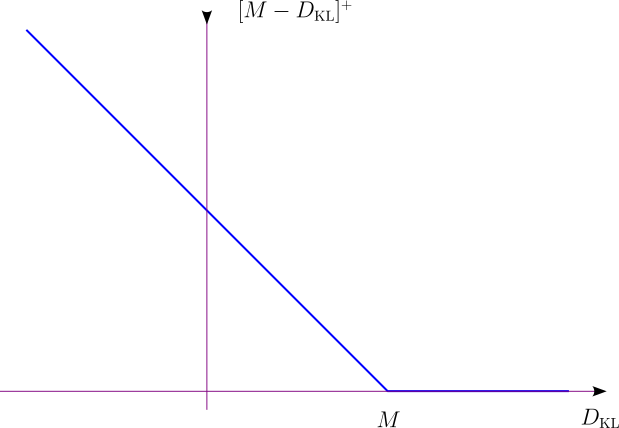
\includegraphics[width=\textwidth]{./assets/hard_constraints.pdf}
    \caption{The hard constraints function $[M - D_{\mathrm{KL}}]^{+}$ of KL divergence in LRAAD}
    \label{fig:hard_constraints}
  \end{minipage}
  \hfill
  \begin{minipage}{0.45\textwidth}
    \centering
    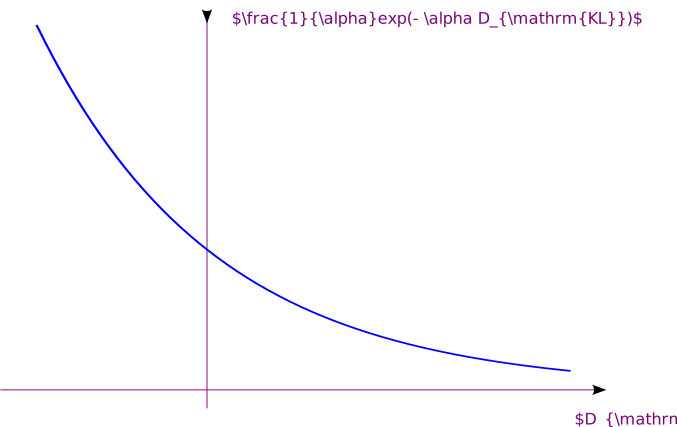
\includegraphics[width=\textwidth]{./assets/soft_constraints.pdf}
    \caption{The soft constraints function $\frac{1}{\alpha}exp(- \alpha D_{\mathrm{KL}})$ of KL divergence in Soft-LRAAD}
    \label{fig:soft_constraints}
  \end{minipage}
\end{figure}

\subsection{软约束损失}

Soft-LRAAD方法中的软约束损失是对LRAAD方法的重要改进之一。LRAAD方法使用硬约束来控制生成图像的KL散度上限,这导致了模型在潜在空间中难以有效区分正常数据和异常数据,同时也可能造成训练不稳定的问题。为了解决这些挑战,Soft-LRAAD引入了软约束损失,通过使用一个平滑的函数来逼近KL散度的上限约束损失,从而缓解了硬约束带来的问题。

为了克服硬约束的缺点,Soft-LRAAD方法引入了软约束损失。软约束损失函数的形式为$\frac{1}{\alpha}\exp(- \alpha D_{\mathrm{KL}}(x))$,其中$\alpha$是一个可调节的超参数。相比于硬约束,软约束的函数图像呈现出平滑递减的趋势,这样的设计使得损失在KL散度接近阈值时依旧缓慢降低,而不是硬约束那样保持不变,这样可以使得生成图像的KL散度可以变大,但又不至于无穷大。通过这种方式,Soft-LRAAD方法能够更好地保持生成图像的质量,同时提高模型的异常检测性能。

与的LRAAD方法不同,Soft-LRAAD采用了软约束的方式来处理KL散度项,使得模型在训练时对KL散度的惩罚更加灵活。具体来说,Soft-LRAAD的编码器损失函数$\mathcal{L}_{\mathrm{E}}$和生成器损失函数$\mathcal{L}_{\mathrm{D}}$分别定义如下:

\begin{equation}
  \mathcal{L}_{\mathrm{E}}=-ELBO(x) + \frac{1}{\alpha}exp(- \alpha D_{\mathrm{KL}}(x^\prime)) + \frac{1}{\alpha}exp(-\alpha D_{\mathrm{KL}}(x^{\prime\prime}))
\end{equation}

\begin{equation}
  \mathcal{L}_{\text {G}}=-ELBO(x) + D_\mathrm{KL}(x^\prime) + D_\mathrm{KL}(x^{\prime\prime}))
\end{equation}

其中,$\alpha$一个可调节的超参数,用于控制软约束项的影响程度。

对于KL散度项,加一个重构损失项,这样可以更好地保持生成图像的质量,同时提高模型的异常检测性能。通过这种方式,Soft-LRAAD方法能够更好地区分正常数据和异常数据,提高异常检测的准确性和鲁棒性。其公式如下所示。

\begin{equation} \label{eq:encoder_loss}
  \mathcal{L}_{\mathrm{E}}=-ELBO(x) + \frac{1}{\alpha}exp(\alpha ELBO(x^\prime)) + \frac{1}{\alpha}exp(\alpha ELBO(x^{\prime\prime}))
\end{equation}

\begin{equation} \label{eq:decoder_loss}
  \mathcal{L}_{\text {G}}=-ELBO(x) - ELBO(x^\prime) - ELBO(x^{\prime\prime}))
\end{equation}

软约束对模型训练的影响主要体现在几个方面。首先,软约束使得潜在变量在潜在空间中分布更加灵活,增强了对正常数据和异常数据的区分能力。其次,软约束的引入有助于模型在训练过程中更加稳定,避免了硬约束可能导致的梯度不连续和训练不稳定问题。最后,通过调节$\alpha$参数,可以灵活控制软约束对KL散度的惩罚力度,进一步优化模型性能。

\subsection{模型训练}

Soft-LRAAD的结构与LRAAD类似,包括编码器$E$、生成器$G$两个部分。编码器$E$负责将输入的梅尔频谱图$x$映射到潜在空间,生成器$G$负责将潜在变量映射回梅尔频谱域,实现频谱图的重建。Soft-LRAAD的整体架构如图\ref{fig:soft_lraad}所示。

Soft-LRAAD的训练过程主要包括编码器$E$和生成器$G$的训练。具体的训练算法如Algorithm 1所示。Soft-LRAAD的训练与LRAAD类似,编码器与生成器以对抗的方式进行训练,通过最小化编码器和生成器的损失函数来优化模型参数。通过交替训练编码器和生成器,Soft-LRAAD模型的编码器能更好地区分正常数据和异常数据,生成器能更好地重建输入的频谱图,从而提高异常检测的准确性和鲁棒性。

\begin{table}[H]
    \centering
    \begin{tabular}{l}
        \toprule
        \label{tab:training}
        {\textbf{Algorithm 1} Training Soft-LRAAD model} \\
        \midrule
        1: Initialize network parameters \\
        2: \quad {\textbf{For} number of epochs \textbf{do}} \\
        3: \quad\quad Random mini-batch $X$ from dataset \\
        4: \quad\quad Compute latent representation of $X$: $Z = E(X)$ \\
        5: \quad\quad Sample $Z_p$ from prior distribution $p(z)=\mathcal{N}(0, I)$ \\
        6: \quad\quad Compute reconstructed spectrogram of $Z$ and $Z_p$: $X^\prime = G(Z)$, $X^{\prime\prime} = G(Z_p)$ \\
        7: \quad\quad Compute latent representation of $X^\prime$ and $X^{\prime\prime}$: $Z^\prime = E(X^\prime)$, $Z^{\prime\prime} = E(X^{\prime\prime})$ \\
        8: \quad\quad Compute Encoder loss $\mathcal{L}_E$ according to Eq. \ref{eq:encoder_loss} \\
        9: \quad\quad Update Encoder parameters by minimizing $\mathcal{L}_E$ \\
        10: \quad\quad Compute Generator loss $\mathcal{L}_G$ according to Eq. \ref{eq:decoder_loss} \\
        11: \quad\quad Update Generator parameters by minimizing $\mathcal{L}_G$ \\
        12: \quad {\textbf{End For}} \\
        \bottomrule
    \end{tabular}
\end{table}




\subsection{异常检测}

我们采用重构误差和 KL 散度之和作为异常分数。重构误差衡量生成频谱图与原始输入频谱图之间的差异,而 KL 散度则衡量潜在表示与标准正态分布之间的差异。对于正常数据,其重构误差较小,潜在表示接近标准正态分布;而对于异常数据,其重构误差较大,潜在表示远离标准正态分布。通过结合这两个指标,模型能够更准确地识别异常数据。异常分数定义的数学表达式如下:

% \begin{equation}
% \mathcal{A}(x)=\left\|x-G\left(E(x)\right)\right\|^2 + D_{\mathrm{KL}}(x)
% \end{equation}
\begin{equation}
\mathcal{A}(x)=\|x-G(E(x))\|^2+D_{\mathrm{KL}}(E(x) \| \mathcal{N}(0, I))
\end{equation}

其中,$\mathcal{A}(x)$表示输入频谱图$x$的异常分数,$E(x)$表示输入频谱图$x$的潜在表示,$G(E(x))$表示潜在表示$E(x)$的重构频谱图,$D_{\mathrm{KL}}(E(x) \| \mathcal{N}(0, I))$表示潜在表示$E(x)$与标准正态分布之间的 KL 散度。通过计算异常分数,我们可以对输入频谱图$x$进行异常检测,判断其是否为异常数据。

% \section{实验:Experiments}
\section{Experiments}
本节我们将介绍实验的设置和结果。我们首先介绍实验的数据集和预处理方法,然后详细描述实验的设置和评估指标,最后给出实验结果和分析。

\subsection{Data Preprocessing}

在本研究中,为了确保高压并联电抗器声音信号的异常检测能够获得准确和可靠的结果,对实验数据进行了系统而细致的预处理。数据预处理的质量直接影响到模型的训练效果和检测性能,因此,我们采用了一系列步骤来优化声音信号数据的处理过程。以下是数据预处理的具体步骤:

实验数据来自中国某特高压变电站的高压并联电抗器实测声音数据。这些声音信号是通过安装在变电站内的高灵敏度传感器采集的,录音文件以WAV格式存储,每个文件的采样频率为44.1kHz,持续时间为10秒。由于原始音频文件较长且包含多种工况信息,为了提高数据处理的精度和模型的训练效率,我们将每个录音文件切分为多个长度为1.36秒的音频片段。这种切分方式确保每个片段能够独立反映电抗器的运行状态,并且便于后续的特征提取和模型训练。

为了更好地捕捉声音信号中的特征信息,我们将切分后的音频片段转换为梅尔频谱图(Mel-spectrogram)。梅尔频谱图是一种在横轴上采用Mel刻度、纵轴上表示功率谱的时频表示形式,它能够更符合人类听觉特性地反映声音信号的频谱特征。相比于传统的频谱图,梅尔频谱图能够更有效地聚焦于声音信号的关键频段,增强低频部分的信息,使得信号特征更加显著。

在生成梅尔频谱图后,为了进一步处理和分析信号中的细微变化,我们对梅尔频谱图进行了对数变换。对数变换能够压缩频谱中的幅度动态范围,减弱高频部分的影响,同时突出低频信号的细节信息。这一变换使得频谱数据更加平滑稳定,有助于模型更好地学习声音信号中的异常特征。


\subsection{Experimental Settings}


在训练 Soft-LRAAD模型时,我们需要设置多个超参数来调节模型的性能。例如,编码器和生成器的学习率、损失函数的权重系数(如重构损失、对抗损失、KL 散度损失的权重)、潜在空间的维度大小、软约束系数、训练的迭代次数等。这些超参数的选择对模型的训练和性能具有重要影响,需要通过实验和验证来确定最佳的超参数组合。在实验中,我们采用的超参数设置如Table \ref{tab:params}所示:

\begin{table}
    \centering
    \caption{Soft-LRAAD Model Hyperparameter Settings}
    \label{tab:params}
    \begin{tabular}{lr}
        \toprule
        \textbf{Hyperparameter} & \textbf{Setting} \\
        \midrule
        Latent Space Dimension & 32 \\
        Learning Rate (Encoder) & 0.0002 \\
        Learning Rate (Generator) & 0.0002 \\
        Loss Weight (Reconstruction) & 1 \\
        Loss Weight (Adversarial) & 1 \\
        Loss Weight (KL Divergence) & 1 \\
        Alpha (Soft Constraint Coefficient) & 128$\times $128 \\
        Training Epochs & 100 \\
        Batch Size & 32 \\
        Dataset Split & 80\% Training, 30\% Testing \\
        \bottomrule
    \end{tabular}
\end{table}


% \subsection{评估指标:Evaluation Metrics}
\subsection{Evaluation Metrics}

在本研究中,我们使用了多种评估指标来量化和比较不同异常检测模型的性能,特别是针对高压并联电抗器声音信号的检测效果。这些评估指标包括ROC曲线(Receiver Operating Characteristic Curve)、AUC(Area Under the ROC Curve)值和p-AUC(Partial Area Under the ROC Curve)值。以下是对这些评估指标的详细描述。

\textbf{ROC曲线:}ROC曲线是一种常用的评估二分类模型性能的工具。它通过绘制真阳性率(True Positive Rate, TPR)与假阳性率(False Positive Rate, FPR)之间的关系,直观展示模型在不同阈值下的分类能力。对于异常检测任务,ROC曲线能够反映出模型在识别异常数据(阳性)与正常数据(阴性)之间的平衡情况。一般来说,ROC曲线越接近左上角(即TPR高且FPR低),说明模型的检测性能越好。在本实验中,我们通过对不同模型生成的异常分数设定多个阈值,计算各个阈值下的TPR和FPR,并绘制ROC曲线,从而对比不同模型的异常检测能力。

\textbf{AUC(Area Under the Curve)值:}AUC值是ROC曲线下方的面积,是衡量模型分类效果的一个综合指标。AUC的取值范围在0.5到1之间,其中0.5表示模型的性能与随机分类等同,1表示模型能够完美区分正常数据与异常数据。因此,AUC值越接近1,说明模型在异常检测中的分类能力越强。AUC指标在本实验中被广泛用于比较不同异常检测模型的整体性能。通过计算不同模型的AUC值,我们能够定量分析它们在高压并联电抗器声音信号检测任务中的表现。

\textbf{p-AUC(Partial Area Under the Curve)值:}p-AUC值是对AUC的进一步细化。它关注的是ROC曲线中FPR小于某个特定阈值时的曲线下面积。通常在实际应用中,我们对异常检测模型的要求是,假阳性率应尽可能低。因此,p-AUC值能够更好地反映模型在低FPR区域的性能,即在严格条件下模型的异常检测能力。在本实验中,我们分别计算了FPR小于0.3、0.2和0.1时的p-AUC值。这些p-AUC值能够帮助我们评估模型在不同假阳性率要求下的性能表现,从而更加准确地反映模型在实际应用中的检测能力。


% \subsection{实验结果:Experimental Results}
\subsection{Experimental Results}

本节将详细介绍基于Soft-LRAAD模型在高压并联电抗器声音信号异常检测任务中的实验结果,并与其他传统模型和深度学习模型进行对比分析。我们主要关注模型的检测精度、鲁棒性以及在不同负载条件下的表现。为了量化各模型的性能,本文使用了ROC曲线、AUC值和p-AUC值等评估指标。实验结果显示,Soft-LRAAD模型在多个实验数据集上均表现出优异的检测性能。

Figure \ref{fig:roc_curve}展示了Soft-LRAAD模型与其他模型在异常检测任务上的ROC曲线。实验中,Soft-LRAAD模型的ROC曲线明显优于传统方法和其他深度学习模型,曲线整体上更接近左上角,表明其在不同阈值下均能有效区分正常数据和异常数据。在六个不同的数据集上,Soft-LRAAD模型的ROC曲线始终处于其他模型之上,表现出更高的真阳性率(TPR)和更低的假阳性率(FPR)。这表明,Soft-LRAAD模型在检测电抗器运行中产生的异常声音信号时,能够更准确地识别出异常,并有效降低误报率。

Table \ref{tab:auc}、\ref{tab:p-auc-03}、\ref{tab:p-auc-02}和\ref{tab:p-auc-01}分别展示了不同模型在不同数据集上的AUC值和p-AUC值。从表中可以看出,Soft-LRAAD模型在大多数数据集上均取得了最高的AUC值,表明其在异常检测任务中具有更强的分类能力。此外,Soft-LRAAD模型在FPR小于0.3、0.2和0.1时的p-AUC值也明显优于其他模型,表明其在低FPR区域的性能更加出色。这些结果表明,Soft-LRAAD模型在高压并联电抗器声音信号异常检测任务中具有更高的检测精度和鲁棒性,能够更好地识别正常数据和异常数据。

\begin{figure}[H]
    \centering
    \includegraphics[width=\textwidth]{./roc_curve.pdf}
    \caption{ROC Curves of Different Models on Different Datasets}
    \label{fig:roc_curve}
\end{figure}

\begin{table}[H]
    \centering
    \caption{AUC Comparison of Different Models on Different Datasets}
    \begin{tabular}{ccccccc}
        \toprule
        Dataset & CAE & VAE & f-AnoGAN & GANomaly & LRAAD & Soft-LRAAD(Our) \\
        \midrule
        Dataset1 & 0.8975 & 0.8662 & 0.8400 & 0.8966 & 0.9361 & \textbf{0.9742} \\
        Dataset2 & 0.8911 & 0.8652 & 0.8560 & 0.9195 & 0.9475 & \textbf{0.9755} \\
        Dataset3 & 0.9266 & 0.8958 & 0.8662 & 0.9266 & 0.9607 & \textbf{0.9851} \\
        Dataset4 & 0.9087 & 0.8868 & 0.8654 & 0.9333 & 0.9626 & \textbf{0.9788} \\
        Dataset5 & 0.8962 & 0.8965 & 0.8910 & 0.9511 & 0.9721 & \textbf{0.9975} \\
        Dataset6 & 0.8523 & 0.8178 & 0.8126 & 0.8270 & 0.8674 & \textbf{0.9782} \\
        \bottomrule
    \end{tabular}
    \label{tab:auc}
\end{table}


\begin{table}[H]
    \centering
    \caption{p-AUC Comparison of Different Models on Different Datasets (FPR<0.3)}
    \begin{tabular}{ccccccc}
        \toprule
        Dataset & CAE & VAE & f-AnoGAN & GANomaly & LRAAD & Soft-LRAAD(Our) \\
        \midrule
        Dataset1 & 0.6664 & 0.5824 & 0.5161 & 0.7232 & 0.7930 & \textbf{0.9162} \\
        Dataset2 & 0.6394 & 0.5559 & 0.5487 & 0.7843 & 0.8430 & \textbf{0.9152} \\
        Dataset3 & 0.7605 & 0.6576 & 0.5935 & 0.8076 & 0.8639 & \textbf{0.9538} \\
        Dataset4 & 0.6972 & 0.6252 & 0.5790 & 0.8164 & 0.8342 & \textbf{0.9118} \\
        Dataset5 & 0.6529 & 0.6569 & 0.6423 & 0.8705 & \textbf{0.8866} & 0.8794 \\
        Dataset6 & 0.5262 & 0.4656 & 0.4589 & 0.5243 & 0.6335 & \textbf{0.9377} \\
        \bottomrule
    \end{tabular}
    \label{tab:p-auc-03}
\end{table}

\begin{table}[H]
    \centering
    \caption{p-AUC Comparison of Different Models on Different Datasets (FPR<0.2)}
    \begin{tabular}{ccccccc}
        \toprule
        Dataset & CAE & VAE & f-AnoGAN & GANomaly & LRAAD & Soft-LRAAD(Our) \\
        \midrule
        Dataset1 & 0.5431 & 0.4503 & 0.3809 & 0.6417 & 0.7078 & \textbf{0.8706} \\
        Dataset2 & 0.5355 & 0.4192 & 0.4037 & 0.7324 & 0.7865 & \textbf{0.8798} \\
        Dataset3 & 0.7041 & 0.5225 & 0.4598 & 0.7496 & 0.8176 & \textbf{0.9399} \\
        Dataset4 & 0.6142 & 0.5014 & 0.4532 & 0.7609 & 0.8173 & \textbf{0.9108} \\
        Dataset5 & 0.5465 & 0.5390 & 0.5371 & \textbf{0.8332} & 0.8115 & 0.8306 \\
        Dataset6 & 0.3801 & 0.3190 & 0.3227 & 0.3935 & 0.5377 & \textbf{0.9097} \\
        \bottomrule
    \end{tabular}
    \label{tab:p-auc-02}
\end{table}

\begin{table}[H]
    \centering
    \caption{p-AUC Comparison of Different Models on Different Datasets (FPR<0.1)}
    \begin{tabular}{ccccccc}
        \toprule
        Dataset & CAE & VAE & f-AnoGAN & GANomaly & LRAAD & Soft-LRAAD(Our) \\
        \midrule
        Dataset1 & 0.3640 & 0.2736 & 0.2261 & 0.5268 & 0.5629 & \textbf{0.8279} \\
        Dataset2 & 0.4405 & 0.2472 & 0.2318 & 0.6353 & 0.6658 & \textbf{0.8068} \\
        Dataset3 & 0.6024 & 0.3372 & 0.2651 & 0.6810 & 0.7020 & \textbf{0.9167} \\
        Dataset4 & 0.5487 & 0.3345 & 0.3136 & 0.6635 & 0.6993 & \textbf{0.8059} \\
        Dataset5 & 0.4090 & 0.3700 & 0.3964 & \textbf{0.7626} & 0.7400 & 0.6544 \\
        Dataset6 & 0.2168 & 0.1566 & 0.1624 & 0.2330 & 0.3791 & \textbf{0.8936} \\
        \bottomrule
    \end{tabular}
    \label{tab:p-auc-01}
\end{table}

%\begin{figure}
%  \centering
%  \includegraphics[width=0.45\linewidth]{./experiments/ssva1/roc_curve.pdf}
%  \hfill
%  \includegraphics[width=0.45\linewidth]{./experiments/ssva2/roc_curve.pdf}
%  \hfill
%  \includegraphics[width=0.45\linewidth]{./experiments/ssva3/roc_curve.pdf}
%  \hfill
%  \includegraphics[width=0.45\linewidth]{./experiments/ssva4/roc_curve.pdf}
%  \hfill
%  \includegraphics[width=0.45\linewidth]{./experiments/ssva5/roc_curve.pdf}
%  \hfill
%  \includegraphics[width=0.45\linewidth]{./experiments/ssva6/roc_curve.pdf}
%\end{figure}



%\subsection{Soft-LRAAD for Feature Extraction}
%
%对于声学特征提取任务,目前主要包括两种方法:基于手工特征的方法和基于深度学习的方法。基于手工特征的方法需要人工设计特征提取器,提取声学信号的频谱、MFCC等特征,然后使用传统的分类器进行分类。这种方法需要大量的领域知识和经验,且往往无法充分挖掘数据的潜在特征。基于深度学习的方法则可以自动学习特征表示,无需人工干预,能够更好地挖掘数据的潜在特征,提高分类性能。
%
%声学特征的手工特征提取方法主要包括时域特征、频域特征和时频域特征。时域特征主要包括时域波形、短时能量、过零率等;频域特征主要包括频谱、功率谱、梅尔频谱等;时频域特征主要包括MFCC、STFT等。时域和频域特征提取的声学信息量较小,往往存在很多的信息丢失,难以充分挖掘数据的潜在特征。而时频域特征提取方法则能够更好地反映声学信号的频谱特征,提高特征的表达能力。我们可以从声音信号的时频域特征很好地重构回原始的音频波形,而时域和频域特征则很难做到这一点,说明时频域特征更具有表达能力,具备原始波形的更多特征信息。
%
%对于深度学习方法,我们认为如果特征能够很好重构回原始数据,那么这个特征就包含了原始数据的更多特征信息,具有更好的表达能力。因此,自编码器是一个很好的特征提取器,它可以通过学习数据的潜在表示来提取数据的特征,从而实现数据的降维和特征提取。
%
%对于Soft-LRAAD模型,其编码器和解码器的优化过程都进行了重构误差损失的优化,而且编码器的优化过程还使得训练数据的潜在表示更接近先验分布,而生成数据的潜在表示则偏离先验分布。这种优化过程使得编码器不仅学习到了更好的特征表示,还学习到了声音是否为正常数据的信息。因此,我们可以将Soft-LRAAD模型的编码器作为特征提取器,用于提取声学信号的特征。通过将声学信号输入到Soft-LRAAD模型的编码器中,可以得到声学信号的潜在表示,这个潜在表示包含了声学信号正常和异常的特征信息,可以用于后续的分类和识别任务。下图为几种算法的潜在表示的t-SNE可视化结果,可以看出Soft-LRAAD模型的潜在表示能够更好地区分正常数据和异常数据。
%
%
%\begin{figure}
%  \centering
%  \includegraphics[width=0.45\linewidth]{./experiments/autoencoder/ssva2/epoch_49_tsne_latents.pdf}
%  \hfill
%  \includegraphics[width=0.45\linewidth]{./experiments/vae/ssva2/epoch_46_tsne_latent.pdf}
%  \hfill
%  \includegraphics[width=0.45\linewidth]{./experiments/fanogan/ssva2/epoch_15_tsne_latents.pdf}
%  \hfill
%  \includegraphics[width=0.45\linewidth]{./experiments/ganomaly/ssva2/epoch_98_latents.pdf}
%  \hfill
%  \includegraphics[width=0.45\linewidth]{./experiments/lraad/ssva2/epoch_88_tsne_latent.pdf}
%  \hfill
%  \includegraphics[width=0.45\linewidth]{./experiments/improved_lraad/ssva2/epoch_99_tsne_latent.pdf}
%  \label{fig:tsne}
%  \caption{t-SNE Visualization of Latent Representations}
%\end{figure}

\section{Conclusion}

在本研究中,我们提出了一种基于软约束潜在正则化对抗学习的高压并联电抗器声音信号异常检测方法(Soft-LRAAD)。该方法旨在解决现有异常检测技术在面对复杂工况下时的灵敏度和鲁棒性不足的问题。通过引入软约束损失函数,Soft-LRAAD模型在潜在空间中实现了对正常数据和异常数据的更有效区分,并在模型训练的稳定性和检测精度方面取得了显著提升。

实验结果表明,Soft-LRAAD方法在不同负载和工况条件下均表现出优异的异常检测性能。相比于传统的油色谱分析、超声波检测和高频局放检测等方法,Soft-LRAAD不仅提高了检测的实时性和精度,还能够更好地应对复杂电磁环境中的干扰问题。此外,与其他深度学习模型相比,Soft-LRAAD在AUC和p-AUC等指标上取得了更高的分数,显示出其在低假阳性率区域的检测优势。

\bibliography{references}

\end{document}

